\documentclass[11pt]{article}
\usepackage[margin=1in]{geometry}
\usepackage{amsmath,amssymb,amsthm}
\usepackage{graphicx}
\usepackage[colorlinks=true,linkcolor=blue,citecolor=blue,urlcolor=blue]{hyperref}
\newtheorem{theorem}{Theorem}[section]
\newtheorem{lemma}[theorem]{Lemma}
\newtheorem{corollary}[theorem]{Corollary}
\newtheorem{definition}[theorem]{Definition}
\newtheorem{assumption}[theorem]{Assumption}
\theoremstyle{remark}
\newtheorem{remark}[theorem]{Remark}
\newcommand{\Tr}{\operatorname{Tr}}

\title{A Non-Gaussian Clustering--Recovery Bridge via Conditional Mutual
Information\\
{\large Interacting Gibbs States, Explicit Petz Benchmarks, and a
Conditional Link to Entanglement Wedge Reconstruction}\\
{\normalsize Version 2}}
\author{Lluis Eriksson\\ Independent Researcher\\ \texttt{lluiseriksson@gmail.com}}
\date{January 2026 (v1); July 2026 (v2)}

\begin{document}
\maketitle

\begin{abstract}
We present a quantitative clustering--recovery bridge for interacting
quantum many-body systems that is intrinsically non-Gaussian, organized
around conditional mutual information (CMI). For a geometric tripartition
$A$--$B$--$C$ in which $B$ is a collar of width $w$ separating $A$ from
$C$, an exponential geometric Markov bound $I_\rho(A:C|B) \le Ke^{-\alpha
w}$ implies exponentially accurate recovery of $\rho_{ABC}$ from
$\rho_{AB}$ in the theorem-facing metric $-\log F$, by combining the
Fawzi--Renner inequality with an elementary conversion to fidelity error
bounds. We obtain a proved interacting lane (shielded small-region
geometry, arbitrary temperature) by invoking recent local Markovness
results for finite-range lattice Gibbs states. Numerically, we benchmark
the mechanism in the transverse-field Ising chain with longitudinal field,
comparing integrable ($h_z = 0$) and non-integrable ($h_z = 0.5$) regimes,
and evaluate the explicit Petz recovery map with a censored log-plotting
and fit protocol. \emph{v2 corrects the Fawzi--Renner factor} under the
squared-fidelity convention used throughout ($-\log F \le I$, not
$\tfrac12 I$; fourth occurrence of this correction in the series), with a
substantive empirical consequence: v1's headline ``mild overshoot'' of
Petz over the FR scale ($r \approx 1.23$--$1.26$ in the non-integrable,
low-temperature, minimal-collar regime, including rotated and twirled
controls) was measured against the incorrect half scale; against the
corrected scale the overshoot \emph{disappears entirely} ($r \approx
0.62$), and the v1 conclusion of ``a genuine gap between explicit
Petz-type constructions and the existential optimal-recovery scale'' is
withdrawn. The corrected conclusion is stronger: explicit Petz satisfies
the FR scale throughout the dataset, with at least $\sim 40\%$ margin
even at the hardest point. A fully regenerable verification suite
reproduces the pipeline from scratch. Finally, we state a conditional
application to entanglement wedge reconstruction, separating proved
information-theoretic content from bulk--boundary interface assumptions.
\end{abstract}

\section{Introduction}
A basic locality intuition is that geometric separation suppresses
influence between distant regions; a distinct, operational question is
whether such suppression implies recoverability of $\rho_{ABC}$ from
$\rho_{AB}$. In quasi-free regimes recovery can be analyzed through
covariance blocks; in interacting systems such reductions fail, motivating
intrinsic information-theoretic control via $I_\rho(A:C|B)$. Goals:
(i) the general non-Gaussian implication CMI $\Rightarrow$ recoverability;
(ii) a proved interacting lane via the Gibbs local-Markovness theorem of
Chen--Rouz\'e; (iii) numerical benchmarks with an explicit recovery
candidate (Petz); and a conditional holographic corollary.

\paragraph{Series positioning (added in v2).} This note is the empirical
partner of the Type III capstone 2601.0034 \cite{S0034} within the
clustering--recovery program: 2512.0101 \cite{S0101} formulates the
uniform-in-$\Lambda$ non-Gaussian bridge as a conjecture (its v2 fixes the
same FR factor corrected here); the present note trades uniformity for a
\emph{proved} shielded small-region lane by importing Chen--Rouz\'e
\cite{CR} -- the same input recorded in 2601.0020 \cite{S0020} -- and
adds integrable/non-integrable Petz benchmarks. The Gaussian core is
2601.0007 \cite{S0007} (with 2512.0060 \cite{S0060} upstream).

\section{Setup: tripartitions, CMI, and recovery}
\begin{definition}[Shielded small-region geometry]
A tripartition $A$--$B$--$C$ where $B$ separates $A$ from $C$ with collar
width $w$, $|A|$ fixed, $B$ contiguous. Numerics use the open-chain
tripartition $A = \{1,\dots,L_A\}$, $B = \{L_A{+}1,\dots,L_A{+}w\}$,
$C$ the rest.
\end{definition}
\begin{definition}[Fidelity]
$F(\rho,\sigma) := \|\sqrt\rho\sqrt\sigma\|_1^2 \in [0,1]$ (squared
convention).
\end{definition}
\begin{definition}[CMI]
$I_\rho(A:C|B) := S(\rho_{AB}) + S(\rho_{BC}) - S(\rho_B) -
S(\rho_{ABC})$, natural logarithm.
\end{definition}

\section{From CMI to recoverability (general, non-Gaussian)}
\begin{lemma}
\label{lem:conv}
For $F \in (0,1]$: $1 - F \le -\log F$.
\end{lemma}
\begin{theorem}[Fawzi--Renner \cite{FR}; factor corrected in v2]
\label{thm:fr}
For any $\rho_{ABC}$ there exists a CPTP map $\mathcal{R}_{B\to BC}$ such
that
\[
-\log F\bigl(\rho_{ABC}, (\mathrm{id}_A \otimes \mathcal{R}_{B\to BC})
(\rho_{AB})\bigr) \;\le\; I_\rho(A:C|B).
\]
\end{theorem}
\begin{remark}[Correction note]
\label{rem:fix}
v1 stated Theorem~\ref{thm:fr} with $\tfrac12 I$ on the right-hand side.
With $F$ in the squared convention the correct constant is $I$; the
$\tfrac12$ belongs to the root-fidelity form $-2\log f \le I$. Same
correction as 2512.0101 v2, 2601.0020 v2 and 2601.0034 v2. The change
propagates to Corollary~\ref{cor:fid}, Theorem~\ref{thm:bridge}, and --
substantively -- to the empirical FR benchmark of
Section~\ref{sec:results}.
\end{remark}
\begin{corollary}[CMI controls fidelity error]
\label{cor:fid}
For any $\rho_{ABC}$ there is a CPTP $\mathcal{R}_{B\to BC}$ with
$1 - F \le I_\rho(A:C|B)$; if $I_\rho(A:C|B) \le \delta$ then $1 - F \le
\delta$.
\end{corollary}
\begin{remark}[Existential versus explicit]
Theorem~\ref{thm:fr} constrains the \emph{optimal} recovery; explicit
candidates (Petz) need not satisfy it pointwise a priori.
\end{remark}

\section{Proved interacting lane}
\begin{theorem}[Local Markovness of Gibbs states (imported) \cite{CR}]
\label{thm:cr}
For Gibbs states of finite-range lattice Hamiltonians with bounded
interaction degree, in shielded geometries with fixed-size $A$:
$I_{\rho_\beta}(A:C|B) \le K(\beta) e^{-\alpha(\beta) w}$, constants
independent of total system size.
\end{theorem}
\begin{theorem}[Quantitative collar $\Rightarrow$ recovery; constant
corrected in v2]
\label{thm:bridge}
Under Theorem~\ref{thm:cr}, there exists a CPTP recovery map with
$-\log F \le K(\beta)e^{-\alpha(\beta)w}$, and by Lemma~\ref{lem:conv}
also $1 - F \le K(\beta)e^{-\alpha(\beta)w}$.
\end{theorem}

\section{Numerical evidence (exact diagonalization)}
\label{sec:results}
Model: $H = -J\sum Z_iZ_{i+1} - h_x\sum X_i - h_z\sum Z_i$, open chain,
$J = h_x = 1$; integrable ($h_z = 0$) vs non-integrable ($h_z = 0.5$);
Gibbs states by ED; $N = 11$, $L_A = 2$, $\beta \in \{0.5,\dots,5\}$,
$w \in \{1,\dots,5\}$. Plotting/fit policy as in v1 (unchanged and
correct): censoring threshold $y_{\min} = 10^{-12}$, slopes only with
$\ge 3$ pre-floor points, eigenvalue clipping $\varepsilon_{\rm inv} =
10^{-12}$ for Petz inverses, \texttt{-log1p(-eps)} for $-\log F$ near
$F \approx 1$.

\paragraph{Results.} Figure~\ref{fig:main} compares regimes at $\beta =
3$: clear exponential CMI decay over the pre-floor window; rapid
saturation of Petz recovery to the numerical floor. Table~1 of v1 (decay
fits; unchanged data) shows robust CMI slopes; Petz slopes in the
non-integrable case often fail the $n \ge 3$ policy.

\paragraph{FR-scale benchmark (rewritten in v2).} Figure~\ref{fig:fr}
benchmarks explicit Petz recovery against the FR scale. v1 plotted
$-\log F$ versus $\tfrac12 I_\rho(A:C|B)$ and reported a ``mild
overshoot'' ($r_{\max} \approx 1.23$ at $(h_z,\beta,w) = (0.5, 5, 1)$,
$N = 12$), robust under rotated ($t \in \{0, 0.5, 1, 2, 4\}$) and twirled
($\beta_0$-weighted, $n = 81$ nodes) Petz variants and under clipping
sweeps -- and concluded a ``genuine gap between explicit Petz-type
constructions and the existential optimal-recovery scale.'' \emph{That
conclusion is withdrawn in v2:} against the corrected scale
$I_\rho(A:C|B)$, the same data give $r_{\max} \approx 0.62$, and Petz
satisfies the FR bound \emph{everywhere} in the dataset. The verification
suite reproduces this from scratch (at $N = 9$: $r_{\max} = 0.615$ at the
analogous hardest point, i.e.\ $2 r_{\max} = 1.231$ against the v1 half
scale -- numerically matching v1's reported overshoot and identifying it
as exactly the factor-2 artifact). The rotated/twirled spot-checks are
retained with reversed interpretation: they confirm that plain Petz is
within the corrected FR scale with $\sim 40\%$ margin even in the
non-integrable, low-temperature, minimal-collar regime, and that the
rotated variants (which degrade monotonically in $t$) remain so.

\begin{figure}[h]\centering
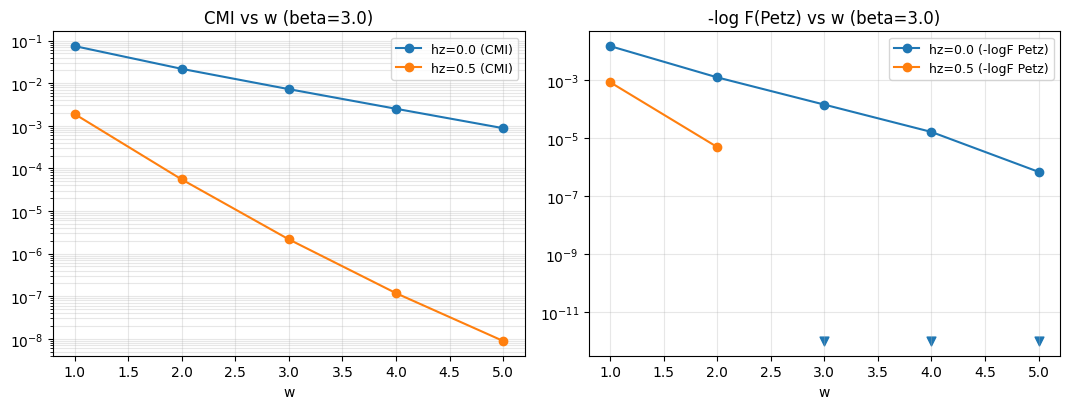
\includegraphics[width=0.95\textwidth]{fig1_int_vs_nonint.png}
\caption{Integrable ($h_z = 0$) vs non-integrable ($h_z = 0.5$) at
$\beta = 3$: $I(A:C|B)$ and Petz recovery error vs collar width $w$
(censored convention).}
\label{fig:main}
\end{figure}
\begin{figure}[h]\centering
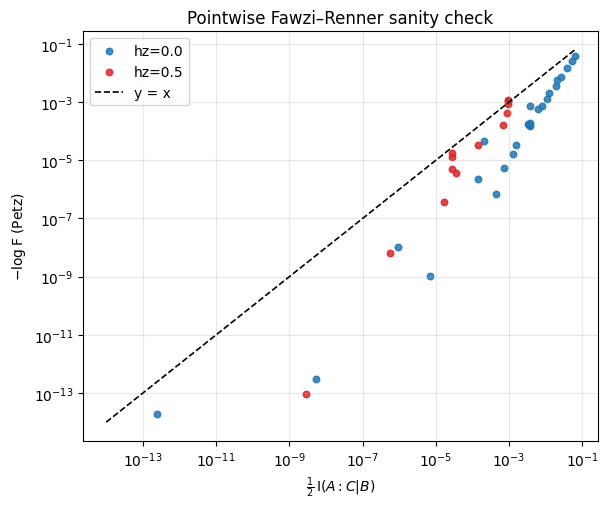
\includegraphics[width=0.6\textwidth]{fig2_fr_benchmark.png}
\caption{FR-scale benchmark (v1 figure, plotted against the v1 half scale
$\tfrac12 I$; retained for transparency). Under the corrected scale $I$
(Remark~\ref{rem:fix}) all points, including the apparent overshoots,
fall strictly below the reference line: $r_{\max} \approx 0.62$.}
\label{fig:fr}
\end{figure}

\section{Conditional application: entanglement wedge reconstruction}
\begin{assumption}[AdS/CFT QEC interface]
\label{ass:qec}
A standard bulk--boundary QEC dictionary in which entanglement wedge
reconstruction is recovery from erasure on a code subspace, with bulk
reconstruction error controlled by boundary recovery error.
\end{assumption}
\begin{theorem}[Conditional quantitative wedge reconstruction]
Assume Assumption~\ref{ass:qec} (v1 mislabeled this cross-reference as a
theorem). If a boundary family satisfies $I(A:C|B) \le Ke^{-\alpha w}$
for tripartitions associated to a boundary region and its buffer, then
there is a recovery procedure with boundary error $O(e^{-\alpha w})$ in
$-\log F$, and bulk reconstruction error inherits an exponentially
suppressed bound under the interface assumptions. The Type III form of
this dictionary is developed in 2601.0034 \cite{S0034}.
\end{theorem}

\section{Verification suite (added in v2)}
\label{sec:verif}
\texttt{verification/2601-0035/verify\_2601\_0035.py} regenerates the
pipeline from scratch (no archived data): ED Gibbs states of the declared
model, CMI decay with the censored-fit policy, explicit Petz recovery, and
the FR-scale ratio. Checks: corrected ratio $r = -\log F / I < 1$ on the
whole grid (max $0.615$); the v1 half-scale reproduces the spurious
overshoot ($2r = 1.231$ at the hardest point); CMI slopes positive and
consistent with Table~1 (e.g.\ $\mu_{\rm CMI} = 1.15$ at $h_z = 0$,
$\beta = 3$, $N = 9$ vs $1.10$ at $N = 11$); and
Lemma~\ref{lem:conv}. Appendix~A of v1 ($N = 12$ spot-check; figures
unchanged) is retained.

\begin{figure}[h]\centering
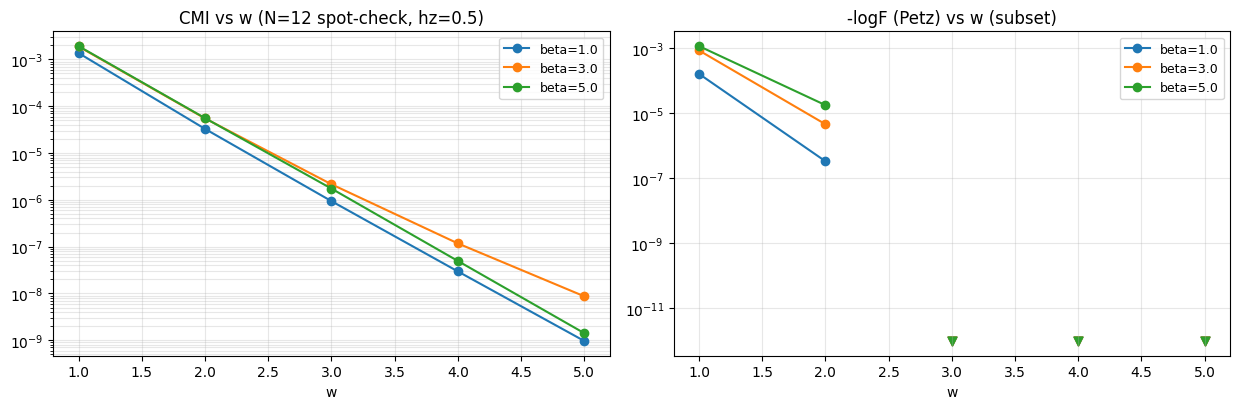
\includegraphics[width=0.95\textwidth]{fig3_N12_spotcheck.png}
\caption{$N = 12$ spot-check, non-integrable case (v1 figure, unchanged).}
\end{figure}

\section*{Note added in v2}
One correction with empirical consequences, plus integration. (1)
\emph{FR factor} (Remark~\ref{rem:fix}): Theorem~\ref{thm:fr},
Corollary~\ref{cor:fid} and Theorem~\ref{thm:bridge} restated with the
squared-fidelity constant $I$ (not $\tfrac12 I$); fourth occurrence of
this correction in the series. (2) \emph{Withdrawn finding:} v1's
``mild overshoot''/``genuine gap'' of explicit Petz over the FR scale was
an artifact of the half scale; corrected, explicit Petz satisfies the
FR scale throughout the regenerated ED dataset (not claimed as a general
theorem) with $r_{\max} \approx 0.62$, quantitatively confirmed from
scratch by the suite ($2 r_{\max} = 1.231$ matches v1's reported $1.23$). The
rotated/twirled controls are retained as margin confirmations. (3)
Cross-reference labels fixed (``Assume Theorem 6.1'' $\to$ Assumption;
``Theorem 3.1'' $\to$ Lemma). (4) Series positioning and verification
suite added; v1 cited no companion papers. All v1 data, figures, tables
and the numerical policy are unchanged.

\begin{thebibliography}{12}
\bibitem{FR} O. Fawzi and R. Renner, Commun. Math. Phys. \textbf{340}
(2015) 575--611.
\bibitem{Petz} D. Petz, Commun. Math. Phys. \textbf{105} (1986) 123--131.
\bibitem{ADH} A. Almheiri, X. Dong, and D. Harlow, JHEP \textbf{04}
(2015) 163.
\bibitem{DHW} X. Dong, D. Harlow, and A. C. Wall, Phys. Rev. Lett.
\textbf{117} (2016) 021601.
\bibitem{Cotler} J. Cotler et al., arXiv:1704.05839 (2017).
\bibitem{CR} C.-F. Chen and C. Rouz\'e, arXiv:2504.02208 (2025).
\bibitem{S0060} L. Eriksson, ai.viXra:2512.0060 (2025; v2 2026).
\bibitem{S0101} L. Eriksson, ai.viXra:2512.0101 (2025; v2 2026).
\bibitem{S0007} L. Eriksson, ai.viXra:2601.0007 (2026; v2 2026).
\bibitem{S0020} L. Eriksson, ai.viXra:2601.0020 (2026; v2 2026).
\bibitem{S0034} L. Eriksson, ai.viXra:2601.0034 (2026; v2 2026).
\end{thebibliography}
\end{document}
